\documentclass[handout]{beamer}

\usepackage{graphicx}
\usepackage{tikz-cd}

\title{EPIT Lecture 5.1\\ The Circle}
\author{Egbert Rijke}
\date{Friday, April 16th 2020}

\setbeamertemplate{caption}{\raggedright\insertcaption\par}

\mathchardef\usc="2D
\newcommand{\N}{\mathbb{N}}
\newcommand{\Z}{\mathbb{Z}}
\newcommand{\UU}{\mathcal{U}}
\newcommand{\brck}[1]{\|#1\|}
\newcommand{\Brck}[1]{\left\|#1\right\|}
\newcommand{\trunc}[2]{\|#2\|_{#1}}
\newcommand{\Trunc}[2]{\left\|#2\right\|_{#1}}
\newcommand{\unit}{\mathbf{1}}
\newcommand{\sphere}[1]{S^{#1}}
\newcommand{\isnull}{\mathsf{is\usc{}null}}
\newcommand{\htpy}{\sim}
\newcommand{\apbinary}{\mathsf{ap\usc{}bin}}
\newcommand{\Glob}{\mathsf{Glob}}
\newcommand{\typeGlob}{\mathsf{type}}
\newcommand{\relGlob}{\mathsf{rel}}
\newcommand{\homGlob}{\mathsf{hom}}
\newcommand{\maphomGlob}{\mathsf{map}}
\newcommand{\cgrhomGlob}{\mathsf{cgr}}
\newcommand{\bihomGlob}{\mathsf{bihom}}
\newcommand{\mapbihomGlob}{\mathsf{map}}
\newcommand{\cgrbihomGlob}{\mathsf{cgr}}
\newcommand{\ct}{\bullet}
\newcommand{\isconstant}[2]{\mathsf{is\usc{}}(#1,#2)\mathsf{\usc{}constant}}
\newcommand{\ap}{\mathsf{ap}}
\newcommand{\interchange}{\mathsf{interchange}}
\newcommand{\refl}{\mathsf{refl}}
\newcommand{\eh}{\mathsf{eckmann\usc{}hilton}}
\newcommand{\blank}{\mathord{\hspace{1pt}\text{--}\hspace{1pt}}}
\newcommand{\EM}{\mathsf{EM}}
\newcommand{\baseS}{\mathsf{base}}
\newcommand{\loopS}{\mathsf{loop}}
\newcommand{\apd}{\mathsf{apd}}
\newcommand{\tr}{\mathsf{tr}}
\newcommand{\idfunc}{\mathsf{id}}
\newcommand{\mulcircle}{\mu}
\newcommand{\basemulcircle}{\mathsf{base\usc{}mul}_{\sphere{1}}}
\newcommand{\loopmulcircle}{\mathsf{loop\usc{}mul}_{\sphere{1}}}
\newcommand{\htpyidcircle}{H}
\newcommand{\basehtpyidcircle}{\alpha}
\newcommand{\loophtpyidcircle}{\beta}
\newcommand{\invcircle}{\mathsf{inv}_{\sphere{1}}}
\newcommand{\evbase}{\mathsf{ev\usc{}base}}
\newcommand{\eqhtpy}{\mathsf{eq\usc{}htpy}}
\newcommand{\apply}[2]{#1(#2)}

\setbeamertemplate{navigation symbols}{}
\setbeamertemplate{footline}[frame number]{}

\begin{document}

\begin{frame}
  \maketitle
\end{frame}

\begin{frame}
  \frametitle{Planning for this afternoon}
  \begin{description}
  \item[14:05-14:30] Part 1. The circle
  \item[14:35-15:00] Part 2. The universal cover of the circle
  \item[15:05-15:30] Part 3. Homotopical constructions of types
  \item[15:35-16:00] Exercise session
  \item[16:05-16:30] Part 4. Homotopy groups of types
  \item[16:35-17:00] Part 5. The real projective spaces
  \item[17:00-17:30] Break
  \item[17:30-18:30] Lecture by Paige North on Directed type theory
  \end{description}
\end{frame}

\begin{frame}[plain]
  \begin{center}
    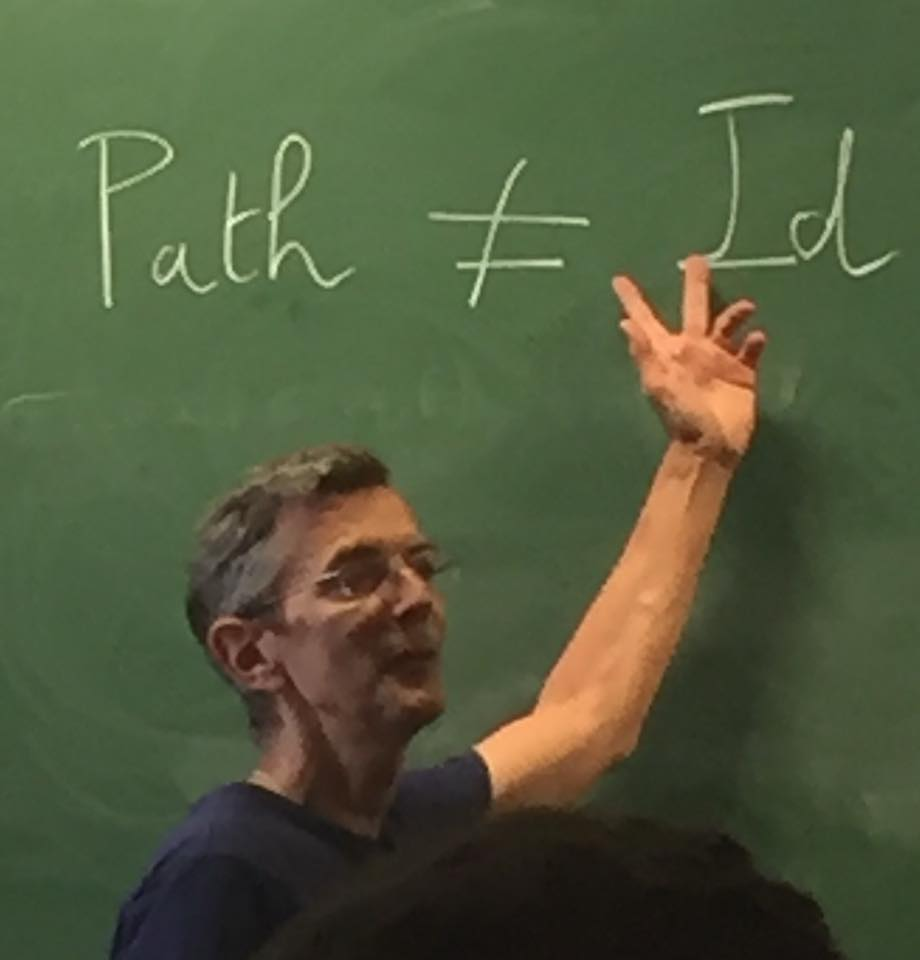
\includegraphics[width=.6\paperwidth]{thierry}
  \end{center}
\end{frame}

\begin{frame}
  The idea of higher inductive types
  \begin{itemize}
  \item Generate types by points and identifications.
    \begin{itemize}
    \item Point constructors
    \item Identity constructors
    \end{itemize}\pause
  \item Equip the type with an induction principle
    \begin{itemize}
    \item Cases for the point constructors
    \item Cases for the identity constructors
    \end{itemize}\pause 
  \item This allows us to study many spaces in type theory that weren't accessible in ordinary MLTT:
    \begin{itemize}
    \item The circle, spheres, projective spaces, CW complexes, Eilenberg-Mac Lane spaces
    \item Pushouts, suspensions, wedge, smash product, 
    \item Homotopy colimits, universal constructions in algebra
    \item Set quotients, groupoid quotients, truncations, Rezk completions, localisations, modalities, spectrifications
    \end{itemize}
  \end{itemize}
\end{frame}

\begin{frame}
  \begin{align*}
    \baseS & : \sphere{1} \\
    \loopS & : \baseS=\baseS
  \end{align*}
\end{frame}

\begin{frame}
  \frametitle{You could have invented higher inductive types}
  An induction principle for a type $X$ tells us how to construct dependent functions
  \begin{equation*}
    \prod_{(x:X)}\apply{P}{x}
  \end{equation*}
  for an arbitrary family $P$ over $X$.\pause
  \begin{itemize}
  \item To find out what the induction principle of $X$ is, the right question to ask is: \\[1em]
    
    {\color{red}Suppose I have a section
      \begin{equation*}
        f:\prod_{(x:X)}\apply{P}{x}.  
      \end{equation*}
      What structure do I get when I apply $f$ to the point constructors and to the identity constructors?}
  \end{itemize}
\end{frame}

\begin{frame}
  \begin{lemma}
    Let $f:\prod_{(x:X)}\apply{P}{x}$, and let $p:x=y$. Then we can construct an identification
    \begin{equation*}
      \apply{\apd_f}{p} : \apply{\tr_P}{p,\apply{f}{x}}=\apply{f}{y}
    \end{equation*}
    in $\apply{P}{y}$. This is the \textbf{dependent action on paths of $f$}.
  \end{lemma}\pause

  \begin{proof}
    By path induction, it suffices to construct an identification
    \begin{equation*}
      \apply{\tr_P}{\refl{},\apply{f}{x}}=\apply{f}{x}.
    \end{equation*}
    However, note that $\apply{\tr_P}{\refl{},\apply{f}{x}} \equiv \apply{f}{x}$, so we have such an identification by reflexivity.
  \end{proof}
\end{frame}

\begin{frame}
  If $f:\prod_{(x:\sphere{1})}\apply{P}{x}$, then we have
  \begin{align*}
    \apply{f}{\baseS} & : \apply{P}{\baseS} \\
    \apply{\apd_f}{\loopS} & : \apply{\tr_P}{\loopS,\apply{f}{\baseS}}= \apply{f}{\baseS}
  \end{align*}\pause
  Therefore we obtain a map
  \begin{equation*}
    \Big(\prod_{(x:\sphere{1})}\apply{P}{x}\Big)\to\Big(\sum_{(u:\apply{P}{\baseS})}\apply{tr_P}{\loopS,u}=u\Big)
  \end{equation*}\pause
  \begin{itemize}
  \item The induction principle of $\sphere{1}$ asserts that this map has a section.
  \item The dependent universal property of $\sphere{1}$ asserts that this map is an equivalence.
  \end{itemize}
\end{frame}

\begin{frame}
  \frametitle{Here's how to use the dependent universal property of $\sphere{1}$}
  Suppose we have
  \begin{align*}
    u & : \apply{P}{\baseS} \\
    p & : \apply{\tr_P}{p,u}=u.
  \end{align*}
  Then there is a unique function $f:\prod_{(x:\sphere{1})}\apply{P}{x}$ equipped with\pause
  \begin{itemize}
  \item an identification
    \begin{equation*}
      \alpha : \apply{f}{\baseS} = u
    \end{equation*}\pause
  \item an identification $\beta$ witnessing that the square
    \begin{equation*}
      \begin{tikzcd}[ampersand replacement=\&,column sep=6em]
        \apply{\tr_P}{\loopS,\apply{f}{\baseS}} \arrow[d,equals,swap,"\apply{apd_f}{\loopS}"] \arrow[r,equals,"\apply{\ap_{\apply{\tr_P}{\loopS}}}{\alpha}"] \& \apply{\tr_P}{\loopS,u} \arrow[d,equals,"p"] \\
        \apply{f}{\baseS} \arrow[r,equals,swap,"\alpha"] \& u
      \end{tikzcd}
    \end{equation*}
    commutes.
  \end{itemize}
\end{frame}

\begin{frame}
  \begin{theorem}
    For any type $Y$, the map
    \begin{equation*}
      (\sphere{1}\to Y)\to \sum_{(y:Y)}y=y
    \end{equation*}
    given by $f\mapsto (\apply{f}{\baseS},\apply{\ap_f}{\loopS})$ is an equivalence.\\[1em]

    The type $\sum_{(y:Y)}y=y$ is also called the \textbf{free loop space} of $Y$.
  \end{theorem}
\end{frame}

\begin{frame}
  \frametitle{Here's how to use the universal property of $\sphere{1}$}
  For any $y:Y$ equipped with $q:y=y$, there is a unique map $f:\sphere{1}\to Y$ equipped with
  \begin{itemize}
  \item an identification $\alpha:\apply{f}{\baseS}=y$
  \item an identification $\beta$ witnessing that the square
    \begin{equation*}
      \begin{tikzcd}[ampersand replacement=\&]
        \apply{f}{\baseS} \arrow[d,equals,swap,"\apply{\ap_f}{\loopS}"] \arrow[r,equals,"\alpha"] \& y \arrow[d,equals,"q"] \\
        \apply{f}{\baseS} \arrow[r,swap,equals,"\alpha"] \& y
      \end{tikzcd}
    \end{equation*}
    commutes.
  \end{itemize}
\end{frame}

\begin{frame}
  \begin{theorem}
    There is a multiplication operation
    \begin{equation*}
      \mu : \sphere{1}\to(\sphere{1}\to\sphere{1})
    \end{equation*}
    that satisfies
    \begin{align*}
      \apply{\mu}{\baseS,y} & = y \\
      \apply{\mu}{x,\baseS} & = x
    \end{align*}
    In particular, it follows that
    \begin{equation*}
      \apply{\mu}{\baseS,\blank} \qquad\text{and}\qquad\apply{\mu}{\blank,\baseS}
    \end{equation*}
    are equivalences.
  \end{theorem}
\end{frame}

\begin{frame}
  \frametitle{Construction of the complex multiplication on $\sphere{1}$}
  We define $\mu:\sphere{1}\to(\sphere{1}\to\sphere{1})$ by the universal property of the circle to be the unique map equipped with
  \begin{itemize}
  \item an identification
    \begin{equation*}
      \basemulcircle : \apply{\mu}{\baseS} = \idfunc
    \end{equation*}
  \item and an identification $\loopS\usc{}\mu$ witnessing that the square
    \begin{equation*}
      \begin{tikzcd}[column sep=huge,ampersand replacement=\&]
        \apply{\mulcircle}{\baseS} \arrow[r,equals,"\basemulcircle"] \arrow[d,equals,swap,"\apply{\ap_{\mulcircle}}{\loopS}"] \& \idfunc \arrow[d,equals,"\apply{\eqhtpy}{\htpyidcircle}"] \\
        \apply{\mulcircle}{\baseS} \arrow[r,equals,swap,"\basemulcircle"] \& \idfunc
      \end{tikzcd}
    \end{equation*}
    where the homotopy $H:\idfunc\htpy\idfunc$ is to be defined.
  \end{itemize}
\end{frame}

\begin{frame}
  It remains to construct $H:\idfunc\htpy\idfunc$, i.e., a dependent function
  \begin{equation*}
    H:\prod_{(x:\sphere{1})}x=x.
  \end{equation*}
  By the dependent universal property of $\sphere{1}$ with $\apply{P}{x}:=(x=x)$, we can define $H$ to be the unique dependent function equipped with
  \begin{itemize}
  \item an identification $\alpha:\apply{H}{\baseS}=\loopS$.
  \item an identification $\beta$ witnessing that the square
    \begin{equation*}
      \begin{tikzcd}[column sep=8em,ampersand replacement=\&]
        \apply{\tr_{P}}{\loopS,\apply{\htpyidcircle}{\baseS}} \arrow[r,equals,"\apply{\ap_{\apply{\tr_{P}}{\loopS}}}{\basehtpyidcircle}"] \arrow[d,equals,swap,"\apply{\apd_{\htpyidcircle}}{\loopS}"] \& \apply{\tr_{P}}{\loopS,\loopS} \arrow[d,equals,"\gamma"] \\
        \apply{\htpyidcircle}{\baseS} \arrow[r,equals,swap,"\basehtpyidcircle"] \& \loopS
      \end{tikzcd}
    \end{equation*}
    where $\gamma:\apply{\tr_P}{\loopS,\loopS}=\loopS$ is to be defined.
  \end{itemize}
\end{frame}

\begin{frame}
  It remains to construct $\gamma:\apply{\tr_P}{\loopS,\loopS}=\loopS$.
  \begin{itemize}
  \item Observation: There is a function
    \begin{equation*}
      (p\bullet r = q \bullet p) \to (\apply{tr_P}{p,q}=r)
    \end{equation*}
    for any $p:\baseS=x$, $q:\baseS=\baseS$, and $r:x=x$. \\[1em]

    Proof. By path induction on $p$. 
  \end{itemize}\pause
  It follows that there is a function
  \begin{equation*}
    f:(\loopS\bullet\loopS = \loopS\bullet\loopS)\to (\apply{\tr_P}{\loopS,\loopS}=\loopS).
  \end{equation*}
  Therefore we define $\gamma:=\apply{f}{\refl}$.\hfill$\square$
\end{frame}

\begin{frame}
  \frametitle{Exercises}
  \begin{enumerate}
  \item Let $X,Y$ be types, and define the family $P$ over $X$ by
    \begin{equation*}
      \apply{P}{x}:=Y.
    \end{equation*}
    show that
    \begin{equation*}
      \apply{\tr_P}{p,y}=y
    \end{equation*}
    for all $y:Y$ and any identification $p$ in $X$.
  \item Show that $\brck{x=y}$ for any $x,y:\sphere{1}$.
  \item Show that $X$ is a set if and only if the map
    \begin{equation*}
      (\sphere{1}\to X)\to X
    \end{equation*}
    given by $f\mapsto \apply{f}{\baseS}$ is an equivalence.
  \item Show that multiplication on $\sphere{1}$ is commutative and associative.
  \end{enumerate}
\end{frame}

\end{document}
